%%\title{Conventions}
%  Changed by: Chris ISELIN, 27-Mar-1997 
%  Changed by: Hans Grote, 25-Sep-2002 
%  Changed by: Ghislain ROY, 24-Jan-2014

\chapter{Conventions}
\label{chap:conventions}
\index{conventions}


\section{Reference System}
\label{sec:reference}
\index{reference!system}
\index{reference!orbit}
\index{local coordinates}
\index{coordinates!local}
The accelerator and/or beam line to be studied is described as a
sequence of beam elements placed sequentially along a reference
orbit. 
The reference orbit is the path of a charged particle having the
central design momentum of the accelerator through idealised magnets
with no fringe fields (see Figure~\ref{F-REF}). 

%% \begin{figure}[h!]
%%   \centering
%% 	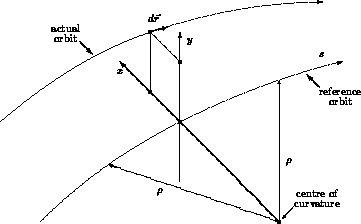
\includegraphics{figures/local_reference.png}
%%   \caption{\href{local}{Local Reference System}}%{\textbf{Figure 1:} Local Reference System}}
%% \end{figure}


\begin{figure}[htb]
\centering
\setlength{\unitlength}{1pt}
\begin{picture}(400,250)
% axes
\thicklines
\put(180,40){\vector(0,1){150}}
\put(190,180){\makebox(0,0){\(y\)}}
\put(280,0){\vector(-1,1){160}}
\put(120,150){\makebox(0,0){\(x\)}}
\thinlines
\put(180,100){\circle*{4}}
% coordinates
\put(150,130){\line(0,1){60}}
\put(180,160){\line(-1,1){30}}
\put(150,130){\circle*{4}}
\put(150,190){\circle*{4}}
\put(180,160){\circle*{4}}
% radii of curvature and centre
\put(280,0){\vector(-3,1){172}}
\put(160,30){\makebox(0,0){\(\rho\)}}
\put(280,0){\vector(0,1){142}}
\put(290,60){\makebox(0,0){\(\rho\)}}
\put(280,0){\circle*{4}}
\put(295,15){\vector(-1,-1){12}}
\put(295,15){\makebox(0,0)[bl]{\shortstack{centre of \\curvature}}}
% actual orbit
\thicklines
\bezier{150}(0,100)(75,165)(150,190)
\put(150,190){\vector(3,1){18}}
\put(159,200){\makebox(0,0)[br]{\(d\vec r\)}}
\bezier{150}(150,190)(240,220)(320,220)
\put(320,220){\vector(1,0){4}}
\put(80,180){\vector(1,-1){12}}
\put(80,180){\makebox(0,0)[br]{\shortstack{actual \\orbit}}}
% actual orbit
\bezier{150}(40,0)(100,60)(180,100)
\bezier{150}(180,100)(260,140)(340,160)
\put(340,160){\vector(4,1){4}}
\put(320,165){\makebox{\(s\)}}
\put(320,135){\vector(-1,1){12}}
\put(320,135){\makebox(0,0)[tl]{\shortstack{reference \\orbit}}}
\end{picture}
\caption{Local Reference System}
\label{F-REF}
\end{figure}


The reference orbit consists of a series of straight line segments and
circular arcs. It is defined under the assumption that all elements are
perfectly aligned. The accompanying tripod of the reference orbit spans
a local curvilinear right handed coordinate system \textit{(x,y,s)} The
local \textit{s}-axis is the tangent to the reference orbit. The two
other axes are perpendicular to the reference orbit and are labelled
\textit{x} (in the bend plane) and \textit{y} (perpendicular to the bend
plane).  


\section{Closed Orbit}
\label{sec:closed_orbit}

Due to various errors like misalignment errors, field errors, fringe
fields etc., the closed orbit does not coincide with the reference
orbit. It also changes with the momentum error. The closed orbit is
described with respect to the reference orbit, using the local
reference system (\textit{x, y, s}). It is evaluated including any
nonlinear effects.  

\madx also computes the betatron and synchrotron oscillations with respect
to the closed orbit. Results are given in the local (\textit{x, y,
  s})-system defined by the reference orbit. 



\section{Global Reference System}
\label{sec:global_ref}

The \hyperlink{global}{global reference orbit} of the accelerator is
uniquely defined by the sequence of physical elements. The local
reference system (\textit{x}, \textit{y}, \textit{s}) may thus be
referred to a global Cartesian coordinate system (\textit{X},
\textit{Y}, \textit{Z}) (see Figure~\ref{F-GLOB}). 
The positions between beam elements are numbered 0,\ldots,i,\ldots,n. 
The local reference system  (\textit{x$_i$, y$_i$, s$_i$}) at position
\textit{i}, i.e. the displacement and direction of the reference orbit
with respect to the system (\textit{X}, \textit{Y}, \textit{Z}) are
defined by three displacements  (\textit{X$_i$}, \textit{Y$_i$},
\textit{Z$_i$}) and three angles (\textit{Theta$_i$}, \textit{Phi$_i$},
\textit{Psi$_i$}) 

\begin{figure}[htb]% 1.2
\centering
\setlength{\unitlength}{1pt}
\begin{picture}(400,270)
% global axes
\thicklines
\put(20,150){\vector(2,-1){280}}
\put(290,35){\makebox(0,0){\(Z\)}}
\put(20,100){\vector(3,1){360}}
\put(370,200){\makebox(0,0){\(X\)}}
\put(80,0){\vector(0,1){270}}
\put(70,240){\makebox(0,0){\(Y\)}}
%local axes
\put(133.3,0){\vector(1,3){90}}
\put(213.3,260){\makebox(0,0){\(x\)}}
\put(300,150){\vector(-2,1){180}}
\put(150,215){\makebox(0,0){\(y\)}}
\put(0,100){\vector(2,1){270}}
\put(260,240){\makebox(0,0){\(s\)}}
% projection of s onto ZX
\thinlines
\put(80,120){\circle*{4}}
\put(200,200){\circle*{4}}
\put(0,110){\line(1,0){290}}
\put(300,110){\makebox(0,0)[l]{\shortstack{projection of \(s\) \\
onto \(ZX\)-plane}}}
\put(20,110){\circle*{4}}
\put(50,110){\circle*{4}}
\put(100,110){\circle*{4}}
% displacement of local system
\put(140,140){\line(2,-1){60}}
\put(160,128){\makebox(0,0)[tr]{\(Z\)}}
\put(140,90){\line(3,1){60}}
\put(190,100){\makebox(0,0)[tl]{\(X\)}}
\put(200,110){\line(0,1){90}}
\put(205,140){\makebox(0,0)[l]{\(Y\)}}
\put(140,90){\circle*{4}}
\put(140,140){\circle*{4}}
\put(200,110){\circle*{4}}
% intersection of xy and ZX
\put(130,0){\line(1,1){230}}
\put(135,5){\circle*{4}}
\put(193.3,63.3){\circle*{4}}
\put(240,110){\circle*{4}}
\put(286.7,156.7){\circle*{4}}
\put(335,205){\circle*{4}}
\thicklines
\put(180,20){\vector(-1,1){12}}
\put(180,20){\makebox(0,0)[tl]{\shortstack{intersection of \\
\(xy\) and \(ZX\) planes}}}
% reference orbit
\bezier{80}(140,150)(170,185)(200,200)
\bezier{80}(200,200)(230,215)(260,220)
\put(260,220){\makebox(0,0)[l]{\shortstack{reference \\orbit}}}
% roll angle
\bezier{30}(160,30)(160,40)(150,50)
\put(152,48){\vector(-1,1){2}}
\put(150,30){\makebox(0,0){\(\psi\)}}
\put(140,30){\makebox(0,0)[br]{roll angle}}
% pitch angle
\bezier{20}(60,110)(60,120)(55,125)
\put(57,123){\vector(-1,2){2}}
\put(50,118){\makebox(0,0){\(\phi\)}}
\put(40,125){\makebox(0,0)[br]{pitch angle}}
% azimuth
\bezier{20}(130,95)(140,100)(140,110)
\put(140,105){\vector(0,1){5}}
\put(130,105){\makebox(0,0){\(\theta\)}}
\put(115,95){\makebox(0,0)[t]{azimuth}}
\end{picture}
\caption{Global Reference System}
\label{F-GLOB}
\end{figure}



The above quantities are defined more precisely as follows:  
\begin{madlist}
   \ttitem{X} Displacement of the local origin in \textit{X}-direction. 
   \ttitem{Y} Displacement of the local origin in \textit{Y}-direction. 
   \ttitem{Z} Displacement of the local origin in \textit{Z}-direction. 
   \ttitem{THETA} Angle of rotation (azimuth) about the
     global \textit{Y}-axis, between the global \textit{Z}-axis and the
     projection of the reference orbit onto the (\textit{Z},
     \textit{X})-plane. A positive angle THETA forms a right-hand screw
     with the \textit{Y}-axis. 
   \ttitem{PHI} Elevation angle, i.e. the angle between the
     reference orbit and its projection onto the (\textit{Z},
     \textit{X})-plane. A positive angle PHI correspond to increasing
     \textit{Y}. If only horizontal bends are present, the reference
     orbit remains in the (\textit{Z}, \textit{X})-plane. In this case
     PHI is always zero. 
   \ttitem{PSI} Roll angle about the local \textit{s}-axis,
     i.e. the angle between the intersection (\textit{x}, \textit{y})-
     and (\textit{Z}, \textit{X})-planes and the local
     \textit{x}-axis. A positive angle PSI forms a right-hand screw with
     the \textit{s}-axis. 
\end{madlist} 

The angles (THETA, PHI, PSI) are \textbf{not} the Euler angles. The
reference orbit starts at the origin and points by default in the
direction of the positive \textit{Z}-axis. The initial local axes
(\textit{x}, \textit{y}, \textit{s})  coincide with the global axes
(\textit{X}, \textit{Y}, \textit{Z}) in this order. The six quantities
(X$_0$, Y$_0$, Z$_0$, THETA$_0$, PHI$_0$, PSI$_0$) thus all have zero
initial values by default. The program user may however specify
different initial conditions.  

Internally the displacement is described by a vector \textit{V} and the
orientation by a unitary matrix \textit{W}. The column vectors of
\textit{W} are the unit vectors spanning  the local coordinate axes in
the order (\textit{x, y, s}). \textit{V} and \textit{W} have the values:  

\[
V =
 \begin{pmatrix}
  X \\
  Y \\
  Z
 \end{pmatrix}
, \qquad
W=\Theta \Phi \Psi
\]
 where 
\[
\Theta =
 \begin{pmatrix}
  \cos \theta  & 0 &  \sin \theta \\
  0            & 1 &  0 \\
  -\sin \theta & 0 &  \cos \theta
 \end{pmatrix}
, \quad
\Phi =
 \begin{pmatrix}
  1 & 0          &  0 \\
  0 & \cos \phi  &  \sin \phi \\
  0 & -\sin \phi &  \cos \phi
 \end{pmatrix}
, \quad
\Psi =
 \begin{pmatrix}
  \cos \psi &  -\sin \psi & 0 \\
  \sin \psi &  \cos \psi  & 0 \\
  0	    &	0	  & 1 
 \end{pmatrix}
.
\]

The reference orbit should be closed and it should not be twisted. This
means that the displacement of the local reference system must be
periodic with the revolution frequency of the accelerator, while the
position angles must be periodic (modulo \(2\pi\)) with the revolution
frequency. If $\psi$ is not periodic (modulo $2\pi$), coupling effects are
introduced. 
When advancing through a beam element, \madx computes
$V_i$ and $W_i$ by the recurrence relations  
\[
   V_i=W_{i-1}R_i+V_{i-1},
   \qquad
   W_i=W_{i-1}S_i
\]
The vector $R_i$ is the displacement and the matrix
$S_i$ is the rotation of the local reference system  at the
exit of the element \textit{i} with respect to the entrance  of the same
element. The values of $R_i$ and $S_i$ are listed in the:
\href{local_system.html#straight}{straight reference system} 
for each physical element type.  

%% \begin{figure}[h!]
%%   \centering
%% 	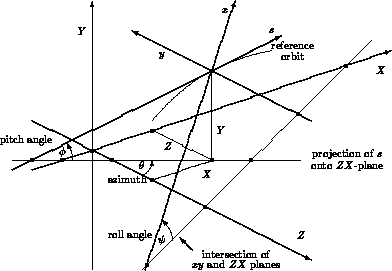
\includegraphics{figures/global.png}
%%   \caption{\href{global}{Global Reference System }}%{\textbf{Figure 1:} Local Reference System}}
%% \end{figure}



\section{Local Reference Systems}
\label{sec:local_ref}

\subsection{\href{straight}{Reference System for Straight Beam
    Elements}} 
\label{subsec:local_straight}
In straight elements the local reference system is simply translated by
the length of the element along the local \textit{s}-axis. 
This is true for  
\begin{itemize}
   \item \href{drift.html}{Drift spaces},\index{drift} 
   \item \href{quadrupole.html}{Quadrupoles},\index{quadrupole} 
   \item \href{sextupole.html}{Sextupoles},\index{sextupole} 
   \item \href{octupole.html}{Octupoles},\index{octupole} 
   \item \href{solenoid.html}{Solenoids},\index{solenoid} 
   \item \href{crabcavity.html}{Crab cavities},\index{crab cavity}
   \item \href{cavity.html}{RF cavities},\index{cavity}\index{RF cavity}
   \item \href{separator.html}{Electrostatic separators},\index{separator}\index{electrostatic separator}
   \item \href{kickers.html}{Closed orbit correctors},\index{corrector} 
   \item \href{monitors.html}{Beam position monitors}.\index{monitor} 
\end{itemize} 

The corresponding \textit{R}, \textit{S} are 
\[
R =
 \begin{pmatrix}
  0 \\
  0 \\
  L
 \end{pmatrix}
, \quad
S =
 \begin{pmatrix}
  1 & 0 &  0 \\
  0 & 1 &  0 \\
  0 & 0 &  1
 \end{pmatrix}
.
\]
A rotation of the element about the \textit{S}-axis has no effect on
\textit{R} and \textit{S}, since the rotations of the reference system
before and after the element cancel.  

%%\begin{center}
%%\includegraphics{null}
%\begin{figure}[H]
%  \centering
%	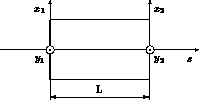
\includegraphics{figures/ref_straight.png}
%  \caption{Reference System for Straight Beam Elements}
%\\\textbf{Figure 1:} Reference System for Straight Beam Elements 
%\end{figure}

%% % picture prepared by ghislain to reproduce the png graphics above.
%% \begin{figure}[htb]
%%   \centering
%%   \setlength{\unitlength}{1pt}
%%   \begin{picture}(200,200)
%%     \thinlines
%%     % s-axis
%%     \put(0,100){\line(1,0){20}}
%%     \put(30,100){\line(1,0){140}}
%%     \put(180,100){\vector(1,0){20}}
%%     \put(200,90){\makebox(0,0){$s$}}
%%     % y-axes
%%     \put(25,100){\circle{10}}
%%     \put(25,100){\circle*{2}}
%%     \put(18,110){\makebox(0,0){$y_1$}}
%%     \put(175,100){\circle{10}}
%%     \put(175,100){\circle*{2}}
%%     \put(182,110){\makebox(0,0){$y_2$}}
%%     % x-axes
%%     \put(25,15){\line(0,1){80}}
%%     \put(25,105){\vector(0,1){80}}
%%     \put(16,180){\makebox(0,0){$x_1$}}
%%     \put(175,15){\line(0,1){80}}
%%     \put(175,105){\vector(0,1){80}}
%%     \put(184,180){\makebox(0,0){$x_2$}}
%%     % length
%%     \put(25,30){\vector(1,0){150}}
%%     \put(175,30){\vector(-1,0){150}}
%%     \put(100,25){\makebox(0,0){$L$}}
%%     % element box
%%     \thicklines
%%     \put(25,50){\line(0,1){45}}
%%     \put(25,105){\line(0,1){45}}
%%     \put(25,150){\line(1,0){150}}
%%     \put(175,150){\line(0,-1){45}}
%%     \put(175,95){\line(0,-1){45}}
%%     \put(175,50){\line(-1,0){150}}
%%   \end{picture}
%%   \caption{Reference System for Straight Beam Elements}
%%   \label{F-REF2}
%% \end{figure}

%% Original picture from MAD-8 manual 
\begin{figure}[ht]
\centering
\setlength{\unitlength}{1pt}
\begin{picture}(400,100)
\thinlines
% axes
\put(150,50){\circle{8}}\put(150,50){\circle*{2}}
\put(140,40){\makebox(0,0){\(y_1\)}}
\put(250,50){\circle{8}}\put(250,50){\circle*{2}}
\put(260,40){\makebox(0,0){\(y_2\)}}
\put(100,50){\line(1,0){46}}
\put(154,50){\line(1,0){92}}
\put(254,50){\vector(1,0){46}}
\put(290,40){\makebox(0,0){\(s\)}}
\put(150,0){\line(0,1){46}}
\put(150,54){\vector(0,1){46}}
\put(140,90){\makebox(0,0){\(x_1\)}}
\put(250,0){\line(0,1){46}}
\put(250,54){\vector(0,1){46}}
\put(260,90){\makebox(0,0){\(x_2\)}}
% magnet outline
\thicklines
\put(150,54){\line(0,1){26}}
\put(150,46){\line(0,-1){26}}
\put(250,54){\line(0,1){26}}
\put(250,46){\line(0,-1){26}}
\put(150,20){\line(1,0){100}}
\put(150,80){\line(1,0){100}}
\put(200,2){\vector(1,0){50}}
\put(200,2){\vector(-1,0){50}}
\put(200,10){\makebox(0,0){L}}
\end{picture}
\caption{Reference System for Straight Beam Elements}
\label{F-DRF}
\end{figure}
 

\subsection{\href{rbend}{Reference System for Bending Magnets}}
\label{subsec:local_rbend}
\href{bend.html}{Bending magnets} have a curved reference orbit. 
For both rectangular and sector bending magnets  
\[
R =
 \begin{pmatrix}
  \rho\,(\cos \alpha - 1) \\
  0 \\
  \rho\,\sin \alpha
 \end{pmatrix}
, \quad
S =
 \begin{pmatrix}
  \cos \alpha & 0 &  -\sin \alpha \\
  0 & 1 &  0 \\
  \sin \alpha & 0 &  \cos \alpha
 \end{pmatrix}
,
\]
where $\alpha$ is the bend angle. 
A positive bend angle represents a bend to the right, i.e. towards
negative \textit{x} values. 
For sector bending magnets, the bend radius is given by $\rho$, and for
rectangular bending magnets it has the value $\rho = L / (2 \sin(\alpha/2))$. 
If the magnet is rotated about the \textit{s}-axis by an angle psi,
\textit{R} and \textit{S} are transformed by  
\[
   \overline{R}=TR,
   \qquad
   \overline{S}=TST^{-1}
\]
where \textit{T} is the orthogonal rotation matrix 
\[
T =
 \begin{pmatrix}
  \cos \psi &  -\sin \psi & 0 \\
  \sin \psi &  \cos \psi  & 0 \\
  0	    &	0	  & 1 
 \end{pmatrix}
.
\]
The special value $\psi = \pi/2$ represents a bend down.  

%% \begin{figure}[htb]
%%   \centering
%% 	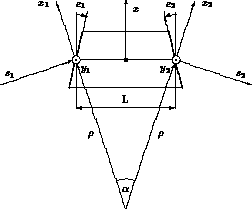
\includegraphics{figures/ref_rbend.png}
%%   \caption{Reference System for Rectangular Bends; The signs of the pole-face rotations are positive as shown.}
%% \end{figure}

%% \begin{figure}[htb]
%%   \centering
%% 	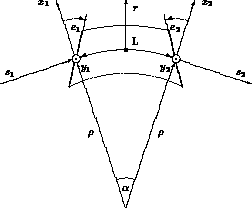
\includegraphics{figures/ref_sbend.png}
%%   \caption{Reference System for Sector Bends; The signs of the pole-face rotations are positive as shown.}
%% \end{figure}
%% \label{local_sbend}

\begin{figure}[htb]
\centering
\setlength{\unitlength}{1pt}
\begin{picture}(400,215)
% axes
\thinlines
\put(150,150){\circle{8}}\put(150,150){\circle*{2}}
\put(160,140){\makebox(0,0){\(y_1\)}}
\put(250,150){\circle{8}}\put(250,150){\circle*{2}}
\put(240,140){\makebox(0,0){\(y_2\)}}
\put(74,124.7){\vector(3,1){72}}
\put(84,135){\makebox(0,0){\(s_1\)}}
\put(254,148.7){\vector(3,-1){72}}
\put(316,135){\makebox(0,0){\(s_2\)}}
\put(200,0){\vector(-1,3){48.7}}
\put(165,75){\makebox(0,0){\(\rho\)}}
\put(148.7,154){\vector(-1,3){18}}
\put(118,206){\makebox(0,0){\(x_1\)}}
\put(200,0){\vector(1,3){48.7}}
\put(235,75){\makebox(0,0){\(\rho\)}}
\put(251.3,154){\vector(1,3){18}}
\put(282,206){\makebox(0,0){\(x_2\)}}
\bezier{20}(190.5,28.5)(200,31.7)(209.5,28.5)
\put(200,20){\makebox(0,0){\(\alpha\)}}
\put(154,150){\line(1,0){92}}
\put(200,150){\circle*{4}}
\put(200,150){\vector(0,1){60}}
\put(210,200){\makebox(0,0){\(x\)}}
\put(150,154){\line(0,1){44}}
\put(150,146){\line(0,-1){46}}
\put(151,154){\line(1,4){11}}
\put(250,154){\line(0,1){44}}
\put(250,146){\line(0,-1){46}}
\put(249,154){\line(-1,4){11}}
% magnet outline
\thicklines
\put(200,102){\vector(-1,0){50}}
\put(200,102){\vector(1,0){50}}
\put(200,110){\makebox(0,0){L}}
\put(151,154){\line(1,4){6}}
\put(149,146){\line(-1,-4){6}}
\put(249,154){\line(-1,4){6}}
\put(251,146){\line(1,-4){6}}
\put(157,178){\line(1,0){86}}
\put(143,122){\line(1,0){114}}
\bezier{10}(150,195)(155.5,195)(160.9,193.7)
\put(155.5,195){\vector(3,-1){5.4}}
\put(150,205){\makebox(0,0)[l]{\(e_1\)}}
\bezier{10}(250,195)(244.5,195)(239.1,193.7)
\put(244.5,195){\vector(-3,-1){5.4}}
\put(250,205){\makebox(0,0)[r]{\(e_2\)}}
\end{picture}
\caption[Reference System for a Rectangular Bending Magnet]%
{Reference System for a Rectangular Bending Magnet;
the signs of pole-face rotations are positive as shown.}
\label{F-RBND}
\end{figure}
 
\begin{figure}[htb]%                                         3.3
\centering
\setlength{\unitlength}{1pt}
\begin{picture}(400,215)
% axes
\thinlines
\put(150,150){\circle{8}}\put(150,150){\circle*{2}}
\put(160,140){\makebox(0,0){\(y_1\)}}
\put(250,150){\circle{8}}\put(250,150){\circle*{2}}
\put(240,140){\makebox(0,0){\(y_2\)}}
\put(74,124.7){\vector(3,1){72}}
\put(84,135){\makebox(0,0){\(s_1\)}}
\put(254,148.7){\vector(3,-1){72}}
\put(316,135){\makebox(0,0){\(s_2\)}}
\put(200,0){\vector(-1,3){48.7}}
\put(165,75){\makebox(0,0){\(\rho\)}}
\put(148.7,154){\vector(-1,3){18}}
\put(118,206){\makebox(0,0){\(x_1\)}}
\put(200,0){\vector(1,3){48.7}}
\put(235,75){\makebox(0,0){\(\rho\)}}
\put(251.3,154){\vector(1,3){18}}
\put(282,206){\makebox(0,0){\(x_2\)}}
\bezier{20}(190.5,28.5)(200,31.7)(209.5,28.5)
\put(200,20){\makebox(0,0){\(\alpha\)}}
\put(200,158.8){\circle*{4}}
\put(200,158.8){\vector(0,1){50}}
\put(210,200){\makebox(0,0){\(r\)}}
\put(151,154){\line(1,4){10}}
\put(249,154){\line(-1,4){10}}
% magnet outline
\thicklines
\bezier{100}(154,151.3)(200,166.7)(246,151.3)
\put(162,154){\vector(-3,-1){8}}
\put(238,154){\vector(3,-1){8}}
\put(210,168){\makebox(0,0){L}}
\put(151,154){\line(1,4){6}}
\put(149,146){\line(-1,-4){6}}
\put(249,154){\line(-1,4){6}}
\put(251,146){\line(1,-4){6}}
\bezier{90}(157,178)(200,188.4)(243,178)
\bezier{110}(143,122)(200,148.6)(257,122)
\bezier{20}(137.4,187.9)(149.1,191.5)(159.7,188.8)
\put(153.7,190.8){\vector(3,-1){6}}
\put(150,180){\makebox(0,0){\(e_1\)}}
\bezier{20}(262.6,187.9)(250.9,191.5)(240.3,188.8)
\put(246.3,190.8){\vector(-3,-1){6}}
\put(250,180){\makebox(0,0){\(e_2\)}}
\end{picture}
\caption[Reference System for a Sector Bending Magnet]%
{Reference System for a Sector Bending Magnet;
the signs of pole-face rotations are positive as shown.}
\label{F-SBND}
\end{figure}


%\subsection{Marker Elements}
%\href{marker.html}{MARKER} elements do not affect the reference orbit. 
%They are ignored for geometry calculations.  


\section{Sign Conventions for Magnetic Fields}
\label{sec:sign_convention}
The \madx program uses the following Taylor expansion for the field on the
mid-plane $y=0$, described in
\href{bibliography.html#slac75}{SLAC-75}:  
\[
B_y(x,0)=\sum_{n=0}^{\infty} \frac{B_n\,x^n}{n!}
\]
Note the factorial in the denominator. 
The field coefficients have the following meaning: 
\begin{madlist}
   \item[$B_0$] 
     Dipole field, with a positive value in the
     positive $y$ direction; a positive field bends a positively
     charged particle to the right.  
   \item[$B_1$] 
     Quadrupole coefficient
     \( B_1 = ( \partial B_y / \partial x ) \);
     a positive value corresponds to horizontal focussing of a
     positively charged particle. 
   \item[$B_2$] 
     Sextupole coefficient
     \( B_2 =  ( \partial^2 B_y / \partial x^2 ) \). 
   \item[$B_3$] 
     Octupole coefficient
     \( B_3 =  ( \partial^3 B_y / \partial x^3 ) \). 
   \item[\ldots] etc.
\end{madlist} 

Using this expansion and the curvature \textit{h} of the reference
orbit, the longitudinal component of the vector potential to order 4 is:  
\[
\begin{aligned}
A_s =  
&+ B_0\,\Big(x-\frac{hx^2}{2(1+hx)}\Big)&
&+ B_1\,\Big(\frac{1}{2}(x^2-y^2) - \frac{h}{6}x^3 + \frac{h^2}{24}(4x^4-y^4)+\cdots\Big) \\
&+ B_2\,\Big(\frac{1}{6}(x^3-3xy^2) - \frac{h}{24}(x^4-y^4)+\cdots \Big)&
&+ B_3\,\Big(\frac{1}{24}(x^4-6x^2y^2+y^4) \cdots \Big)+\cdots
\end{aligned}
\]
Taking \(\vec{B} = \nabla \times \vec{A}\) in curvilinear coordinates,
the field components can be computed as  
\[
\begin{aligned}
B_x(x,y) = &+ B_1\,\Big(y+\frac{h^2}{6}y^3+\cdots\Big)  &  \\
           &+ B_2\,\Big(xy - \frac{h^3}{6}y^3+\cdots \Big) &+ B_3\,\Big(\frac{1}{6}(3x^2y-y^3)+ \cdots \Big)+\cdots\\
B_y(x,y)=  &+ B_0   &+ B_1\,\Big(x-\frac{h}{2}y^2+\frac{h^2}{2}xy^2+\cdots \Big)\\
           &+ B_2\,\Big(\frac{1}{2}(x^2-y^2)-\frac{h}{2}xy^2+\cdots \Big) &+ B_3\,\Big(\frac{1}{6}(x^3-3xy^2)+ \cdots \Big)+\cdots
\end{aligned}
\]
It can be easily verified that both \(\nabla \times \vec{B}\)
and \(\nabla . \vec{B}\) are zero to the order of the
\(B_3\) term.  

Introducing the magnetic rigidity \(B \rho = p_s / q\) as the
momentum of the particle divided by its charge, the multipole
coefficients are computed as
\[ K_n = q B_n / p_s  =  B_n / B \rho \] 



\section{Variables}
\label{sec:variables}
\subparagraph{ For each variable the physical units are listed in square brackets. }

\subsection{\href{canon}{Canonical Variables Describing Orbits}} 
\label{subsec:tables_canon}
\madx uses the following canonical variables to describe the motion of particles: 
\begin{madlist}
   \ttitem{X} Horizontal position $x$ of the (closed) orbit,
     referred to the ideal orbit [m].    
   \ttitem{PX} Horizontal canonical momentum $p_x$ of the
     (closed) orbit referred to the ideal orbit, divided by the
     reference momentum: $\textrm{PX} = p_x / p_0$, [1].   
   \ttitem{Y} Vertical position $y$ of the (closed) orbit, referred
     to the ideal orbit [m].   
   \ttitem{PY} Vertical canonical momentum $p_y$ of the (closed)
     orbit referred to the ideal orbit, divided by the reference
     momentum: $\textrm{PY} = p_y / p_0$, [1].   
   \ttitem{T} Velocity of light times the negative time difference with
     respect to the reference particle: $\textrm{T} =  - c t$, [m]. A
     positive T means that the particle arrives ahead of the reference
     particle.   
   \ttitem{PT} Energy error, divided by the reference momentum times the
     velocity of light: $\textrm{PT} = \Delta E / p_s c$, [1]. 
     This value is only non-zero when synchrotron motion is
     present. It describes the deviation of the particle from the orbit
     of a particle with the momentum error DELTAP.   
   \ttitem{DELTAP} Difference of the reference momentum and the design
     momentum, divided by the reference momentum: DELTAP =
     $\Delta p / p_0$, [1]. This quantity is used to
     \href{defects.html}{normalize} all element strengths.   
\end{madlist} 

The independent variable is: 
\begin{madlist}
  \ttitem{S} \index{arc length} Arc length \textit{s} along the reference orbit, [m].   
\end{madlist} 

In the limit of fully relativistic particles ($\gamma \gg 1$, $v = c$,
$p c = E$), the variables T, PT used here agree with the
longitudinal variables used in
\href{bibliography.html#transport}{[TRANSPORT]}. This means that T
becomes the negative path length difference, while PT becomes the
fractional momentum error. The reference momentum \textit{p$_s$} must be
constant in order to keep the system canonical.  

\subsection{\href{normal}{Normalised Variables and other Derived Quantities}}
\label{subsec:tables_normal}
\begin{madlist}
  \ttitem{XN} The normalised horizontal displacement 
  $x_n = Re ( E_1^T \, S\, Z )$, [sqrt(m)]
  \ttitem{PXN} The normalised horizontal transverse momentum 
  $p_{xn} = Im ( E_1^T\, S\, Z )$, [sqrt(m)]
  \ttitem{WX} The horizontal Courant-Snyder invariant 
  WX = $x_n^2 + p_{xn}^2$, [m].    
  \ttitem{PHIX} The horizontal phase 
  $\phi_x = -\arctan ( p_{xn} / x_n ) / 2 \pi$, [1]
  \ttitem{YN} The normalised vertical displacement 
  $y_n = Re ( E_2^T \,S\, Z )$, [sqrt(m)]
  \ttitem{PYN} The normalised vertical transverse momentum 
  $p_{yn} = Im ( E_2^T\, S\, Z )$, [sqrt(m)]
  \ttitem{WY} The vertical Courant-Snyder invariant 
  WY = $y_n^2 + p_{yn}^2$, [m]
  \ttitem{PHIY} The vertical phase 
  $\phi_y = - \arctan ( p_{yn} / y_n ) / 2 \pi$, [1]
  \ttitem{TN} The normalised longitudinal displacement 
  $t_n = Re ( E_3^T \,S\, Z )$, [sqrt(m)]
  \ttitem{PTN} The normalised longitudinal transverse momentum 
  $p_{tn} = Im ( E_3^T\, S\, Z )$, [sqrt(m)]
  \ttitem{WT} The longitudinal invariant 
  WT = $t_n^2 + p_{tn}^2$, [m]
  \ttitem{PHIT} The longitudinal phase 
  $\phi_t = - atan ( p_{tn} / t_n ) / 2 \pi$, [1]
\end{madlist} 

In the above formulas \(Z\) is the phase space vector
\[
Z = \left(
\begin{array}{l} x \\ p_x \\ y \\ p_y \\ t \\ p_t
\end{array} \right),
\]
the matrix \textit{S} is the ``symplectic unit matrix'' 
\[
S =
 \begin{pmatrix}
  0 & 1 & 0 & 0 & 0 & 0 \\
  -1 & 0 & 0 & 0 & 0 & 0 \\
  0 & 0 & 0 & 1 & 0 & 0 \\
  0 & 0 & -1 & 0 & 0 & 0 \\
  0 & 0 & 0 & 0 & 0 & 1 \\
  0 & 0 & 0 & 0 & -1 & 0 \\
 \end{pmatrix}
\]
and the vectors \(E_i\) are the three complex eigenvectors.

%% In the above formulas \textit{Z} is the phase space vector
%% \textit{Z = ( x, p$_x$, y, p$_y$, t, p$_t$)$^T$}, the vectors
%% \textit{E$_i$} are the three complex eigenvectors and  
%% the matrix \textit{S} is the ``symplectic unit matrix'' 
%% %%\includegraphics{../equations/S_matrix.gif}
%% %S_matrix
%% \[
%% S =
%%  \begin{pmatrix}
%%   0 & 1 & 0 & 0 & 0 & 0 \\
%%   -1 & 0 & 0 & 0 & 0 & 0 \\
%%   0 & 0 & 0 & 1 & 0 & 0 \\
%%   0 & 0 & -1 & 0 & 0 & 0 \\
%%   0 & 0 & 0 & 0 & 0 & 1 \\
%%   0 & 0 & 0 & 0 & -1 & 0 \\
%%  \end{pmatrix}
%% \]


\subsection{\href{linear}{Linear Lattice Functions (Optical Functions)}} 
\label{subsec:tables_linear}
Several \madx commands refer to linear lattice functions. 

Because \madx uses the canonical momenta ($p_x$, $p_y$) instead of the
slopes ($x'$, $y'$), the definitions of the linear lattice functions
differ slightly from those in \href{bibliography.html#courant}{[Courant
    and Snyder]}. 

Notice that in \madx, PT substitutes DELTAP as longitudinal
variable. 
Dispersive and chromatic functions are hence derivatives with
respects to PT. 
And since PT=BETA*DELTAP, where BETA is the relativistic Lorentz 
factor, those functions given by \madx must be multiplied by BETA a
number of time equal to the order of the derivative to find the
functions given in the litterature. 

The linear lattice functions are known to \madx under the following names:
\begin{madlist}
  \ttitem{BETX} Amplitude function $\beta_x$, [m].   
  \ttitem{ALFX} Correlation function 
  $\alpha_x = - \frac{1}{2} (\partial \beta_x / \partial s)$, [1]   
  \ttitem{MUX} Phase function $\mu_x = \int ds / \beta_x$, [$2 \pi$]
  \ttitem{DX} Dispersion of $x$: $D_x = (\partial x / \partial p_t)$, [m] 
  \ttitem{DPX} Dispersion of $p_x$: $D_{px} = (\partial p_x / \partial p_t) / p_s$, [1] 
  \ttitem{BETY} Amplitude function $\beta_y$, [m]   
  \ttitem{ALFY} Correlation function 
  $\alpha_y = - \frac{1}{2} ( \partial \beta_y / \partial s)$, [1] 
  \ttitem{MUY} Phase function $\mu_y = \int ds / \beta_y$, [$2 \pi$]
  \ttitem{DY} Dispersion of $y$: $D_y = (\partial y / \partial p_t)$, [m] 
  \ttitem{DPY} Dispersion of $p_y$: $D_{py} = ( \partial p_y / \partial p_t) / p_s$, [1] 
  \ttitem{R11, R12, R21, R22} : Coupling Matrix     
\end{madlist}

%  The TWISS table also defines the following expressions which 
%  can be used in plots:
% \begin{itemize}
%   \item  GAMX = (1 + ALFX*ALFX) / BETX, 
%   \item  GAMY = (1 + ALFY*ALFY) / BETY, 
%   \item  SIGX = SQRT(BETX * EX), the vertical r.m.s. half-width of the beam, 
%   \item  SIGY = SQRT(BETY * EY), the vertical r.m.s. half-height of the beam. 
% \end{itemize}


\subsection{\href{chrom}{Chromatic Functions}} 
\label{subsec:tables_chrom}
Several \madx commands refer to the chromatic functions. 

Because \madx uses the canonical momenta ($p_x$, $p_y$) instead of the
slopes ($x'$, $y'$), the definitions of the chromatic functions differ
slightly from those in \href{bibliography.html#montague}{[Montague]}.  

Notice also that in \madx, PT substitutes DELTAP as longitudinal
variable. Dispersive and chromatic functions are hence derivatives with
respects to PT. 
And since PT=BETA*DELTAP, where BETA is the relativistic Lorentz 
factor, those functions given by \madx must be multiplied by BETA a
number of time equal to the order of the derivative to find the
functions given in the litterature. 

The chromatic functions are known to \madx under the following names:

\begin{madlist}
  \ttitem{WX} Chromatic amplitude function $W_x = \sqrt{a_x^2 + b_x^2}$ ,
         [1], where \\
         \[
         b_x = \frac{1}{\beta_x} \frac{\partial \beta_x}{\partial p_t}  ,\qquad
         a_x = \frac{\partial \alpha_x}{\partial p_t} -
         \frac{\alpha_x}{\beta_x}\frac{\partial \beta_x}{\partial p_t}
         \]
         %% the equation used to be the following, which is in contradiction
         %% with MAD8 users' guide and Montague (LEP Note 165) where a and b
         %% are exactly inverted. 
         %% \[
         %% a_x = \frac{1}{\beta_x} \frac{\partial \beta_x}{\partial p_t}  ,\qquad
         %% b_x = \frac{\partial \alpha_x}{\partial p_t} -
         %% \frac{\alpha_x}{\beta_x}\frac{\partial \beta_x}{\partial p_t}
         %% \]
  \ttitem{PHIX} Chromatic phase function $\Phi_x = \arctan (a_x / b_x)$, [$2 \pi$] 
  \ttitem{DMUX} Chromatic derivative of phase function: 
  $DMUX = (\partial \mu_x / \partial p_t)$,  [$2 \pi$]
  \ttitem{DDX} Chromatic derivative of dispersion $D_x$ :  
  $DDX = \frac{1}{2} (\partial^2 x / \partial p_t^2)$, [m]     
  \ttitem{DDPX} Chromatic derivative of dispersion $D_{px}$ : 
  $DDPX = \frac{1}{2} ( \partial^2 p_x / \partial p_t^2 ) / p_s $, [1]
  \ttitem{WY} Chromatic amplitude function $W_y = \sqrt{a_y^2 + b_y^2}$ ,
         [1], where \\
         \[
         b_y = \frac{1}{\beta_y} \frac{\partial \beta_y}{\partial p_t} ,\qquad
         a_y = \frac{\partial \alpha_y}{\partial p_t} -
         \frac{\alpha_y}{\beta_y}\frac{\partial \beta_y}{\partial p_t}
         \]
  \ttitem{PHIY} Chromatic phase function $\Phi_y = \arctan (a_y / b_y)$, [$2 \pi$]
  \ttitem{DMUY} Chromatic derivative of phase function:
  $DMUY = (\partial \mu_y / \partial p_t)$,  [$2 \pi$] 
  \ttitem{DDY} Chromatic derivative of dispersion $D_y$ : 
  $DDY = \frac{1}{2} (\partial^2 y / \partial p_t^2)$, [m]      
  \ttitem{DDPY} Chromatic derivative of dispersion $D_{py}$ : 
  $DDPY = \frac{1}{2} ( \partial^2 p_y / \partial p_t^2 ) / p_s $, [1] 
\end{madlist}

\subsection{\href{summ}{Variables in the SUMM Table}} 
\label{subsec:tables_summ}
After a successful TWISS command a summary table, with name SUMM, is created which
contains the following variables:  
\begin{madlist}
  \ttitem{LENGTH} The length of the machine, [m].     
  \ttitem{ORBIT5} The T ($= c t$, [m]) component of the closed orbit.     
  \ttitem{ALFA} The momentum compaction $\alpha_c$, [1].     
  \ttitem{GAMMATR} The transition energy $\gamma_{tr}$, [1].     
  \ttitem{Q1} The horizontal tune $Q_1$ [1].     
  \ttitem{DQ1} The horizontal chromaticity $dq_1 = \partial Q_1 / \partial p_t$, [1]
  \ttitem{BETXMAX} The largest horizontal $\beta_x$, [m].     
  \ttitem{DXMAX} The largest horizontal dispersion $D_x$, [m].     
  \ttitem{DXRMS} The r.m.s. of the horizontal dispersion $D_x$, [m].     
  \ttitem{XCOMAX} The maximum of the horizontal closed orbit deviation [m].     
  \ttitem{XRMS} The r.m.s. of the horizontal closed orbit deviation [m].     
  \ttitem{Q2} The vertical tune $Q_2$ [1].     
  \ttitem{DQ2} The vertical chromaticity $dq_2 = \partial Q_2 / \partial p_t$, [1]
  \ttitem{BETYMAX} The largest vertical $\beta_y$, [m].     
  \ttitem{DYMAX} The largest vertical dispersion $D_y$, [m].     
  \ttitem{DYRMS} The r.m.s. of the vertical dispersion $D_y$, [m].     
  \ttitem{YCOMAX} The maximum of the vertical closed orbit deviation [m].     
  \ttitem{YCORMS} The r.m.s. of the vertical closed orbit deviation [m].     
  \ttitem{DELTAP} Energy difference, divided by the reference
  momentum times the velocity of light: DELTAP = $\Delta E / p_s c$, [1].
  \ttitem{SYNCH\_1} First synchrotron radiation integral  
  \ttitem{SYNCH\_2} Second synchrotron radiation integral  
  \ttitem{SYNCH\_3} Third synchrotron radiation integral  
  \ttitem{SYNCH\_4} Fourth synchrotron radiation integral  
  \ttitem{SYNCH\_5} Fifth synchrotron radiation integral  
\end{madlist} 

Notice that in \madx, PT substitutes DELTAP as longitudinal
variable. Dispersive and chromatic functions are hence derivatives with
respects to PT.
And since PT=BETA*DELTAP, where BETA is the relativistic Lorentz 
factor, those functions given by \madx must be multiplied by BETA a
number of time equal to the order of the derivative to find the
functions given in the litterature. 

\subsection{\href{track}{Variables in the TRACK Table}} 
\label{subsec:tables_track}
The command RUN writes tables with the following variables: 
\begin{madlist}
  \ttitem{X} Horizontal position $x$ of the orbit, referred to the
  ideal orbit [m].    
  \ttitem{PX} Horizontal canonical momentum $p_x$ of the orbit
  referred to the ideal orbit, divided by the reference momentum.    
  \ttitem{Y} Vertical position $y$ of the orbit, referred to the
  ideal orbit [m].    
  \ttitem{PY} Vertical canonical momentum $p_y$ of the orbit
  referred to the ideal orbit, divided by the reference momentum.    
  \ttitem{T} Velocity of light times the negative time difference with
  respect to the reference particle, $\hbox{\tt T}=-c\Delta t$, [m]. 
  A positive T means that the particle arrives ahead of the reference
  particle.    
  \ttitem{PT} Energy difference, divided by the reference momentum times
  the velocity of light, [1].    
\end{madlist} 

When tracking Lyapunov companions, the TRACK table defines the following
dependent expressions:  
\begin{madlist}
  \ttitem{DISTANCE} the relative Lyapunov distance between the two particles.    
  \ttitem{LYAPUNOV} the estimated Lyapunov Exponent.   
  \ttitem{LOGDIST} the natural logarithm of the relative distance.   
  \ttitem{LOGTURNS} the natural logarithm of the turn number.   
\end{madlist}





\section{Physical Units}
\label{sec:units}
Throughout the computations \madx uses international units from the ``Syst\`eme
International'' (SI). These units are summarised in the
\hyperlink{table}{Units table}.  
\begin{table}[h]
  \caption{Physical Units used by \madx}
  \begin{center}
    \index{length}
    \index{angle}
    \index{quadrupole}
    \index{multipole}
    \index{voltage}
    \index{field}
    \index{electric field}
    \index{frequency}
    \index{RF}
    \index{energy}
    \index{mass}
    \index{momentum}
    \index{current}
    \index{charge}
    \index{impedance}
    \index{emittance}
    \index{power}
    \index{high order modes} 
   \begin{tabular}{|l|l|}
      \hline
      Quantity                & Unit \\
      \hline
      Length                  & m (metres) \\ 
      Angle                   & rad (radians) \\ 
      Quadrupole coefficient  & $m^{-2}$ \\ 
      Multipole coefficient, 2n poles   & $m^{-n}$ \\ 
      Electric voltage        & MV (Megavolts) \\ 
      Electric field strength & MV/m \\ 
      Frequency               & MHz (Megahertz) \\ 
      Phase angles            & $2\pi$ \\ 
      Particle energy         & GeV \\ 
      Particle mass           & GeV/$c^2$ \\ 
      Particle momentum       & GeV/c \\ 
      Beam current            & A (Amp\`eres) \\ 
      Particle charge         & e (elementary charges) \\ 
      Impedance               & M$\Omega$ (Megohms) \\ 
      Emittance               & $\pi$.m mrad \\ % To be checked (Ghislain)
      RF power                & MW (Megawatts) \\ 
      Higher mode loss factor & V/pc \\
      \hline
    \end{tabular}
  \end{center}
\end{table}

%% End of Chapter 'Conventions'
